\documentclass{article}
\usepackage{setspace}\setstretch{1.25} % {\setstretch{1.25} \par}
\usepackage[a4paper,height=25cm,hmargin={2.2cm,2.2cm}]{geometry}
%<--------------------------------------------------------------------------->%
%%% Math %%%
\usepackage{gensymb,amssymb}
\usepackage{mathrsfs,amsmath} % \mathscr{F}
\usepackage{mathtools} % \stackrel{i.i.d.}{\sim} % \substack{-\\-} % \middle
% \usepackage{centernot}
% \usepackage{accents}
\usepackage[makeroom]{cancel}
\newcommand{\two}[2]{\substack{ \text{#1} \\ \text{#2} }}
\newcommand{\raum}{\phantom{=}{\:\,}}
%<--------------------------------------------------------------------------->%
%%% Biblatex %%%
\usepackage[hyperref=true,backend=biber,style=apa,sorting=ynt,backref=false]{biblatex} 
\addbibresource{ref.bib}
%\printbibliography[title = \ctxfr{參考文獻}]
%<--------------------------------------------------------------------------->%
%%% Column %%%
\usepackage{multicol}  % \begin{multicols*}{3}[例外]字\end{multicols*}
\usepackage[english]{babel}
%<--------------------------------------------------------------------------->%
%%% Page # of # %%%
\usepackage{fancyhdr,lastpage}
\pagestyle{fancy}\renewcommand{\headrulewidth}{0pt}\fancyhf{}
\fancyfoot[C]{\footnotesize 第 \thepage\ 頁 / 共 \pageref{LastPage} 頁}
\fancypagestyle{plain}{\renewcommand{\headrulewidth}{0pt}\fancyhf{}
\fancyfoot[C]{\footnotesize 第 \thepage\ 頁 / 共 \pageref{LastPage} 頁}}
%<--------------------------------------------------------------------------->%
%%% Graphics %%%
\usepackage{graphicx}
\renewcommand{\figurename}{圖}
\renewcommand{\tablename}{表}
%<--------------------------------------------------------------------------->%
%%% Hyper Reference %%%
\PassOptionsToPackage{hyphens}{url}\usepackage[hidelinks,colorlinks=true]{hyperref}
\newcommand{\supref}[1]{\ref{#1} (p.\pageref{#1})}
%<--------------------------------------------------------------------------->%
%%% CJK %%%
\usepackage{xeCJK}
\setCJKmainfont{GenWanMin TJ L}
[BoldFont={Noto Sans CJK KR Medium},AutoFakeSlant=0.2]
\setCJKsansfont{Noto Sans CJK KR Medium}
[BoldFont={Noto Sans CJK KR Medium},AutoFakeSlant=0.2]
\setCJKmonofont{Noto Sans Mono CJK KR Regular}
\xeCJKsetup{PunctStyle=kaiming,CheckFullRight=true}
\setlength{\parindent}{2em}
%<--------------------------------------------------------------------------->%
%%% Punctuation width %%%
\xeCJKsetwidth{、}{0.55em}
\xeCJKsetwidth{，}{0.6em}
\xeCJKsetwidth{：}{0.65em}
\xeCJKsetwidth{；}{0.65em}
\xeCJKsetwidth{。}{0.7em}
\xeCJKsetwidth{・}{0.7em}
\xeCJKsetwidth{「」}{0.7em}
\xeCJKsetwidth{『』}{0.7em}
\xeCJKsetwidth{（）}{0.7em}
\xeCJKsetwidth{《》}{0.7em}
%%% Punctuation Kerning %%%
\xeCJKsetkern{」}{（}{0.2em}
\xeCJKsetkern{」}{、}{0.2em}
\xeCJKsetkern{」}{，}{0.2em}
\xeCJKsetkern{」}{。}{0.2em}
\xeCJKsetkern{」}{；}{0.2em}
\xeCJKsetkern{」}{：}{0.2em}
\xeCJKsetkern{、}{「}{0.4em}
\xeCJKsetkern{、}{（}{0.4em}
\xeCJKsetkern{。}{《}{0.2em}
\xeCJKsetkern{。}{「}{0.4em}
\xeCJKsetkern{。}{」}{0.2em}
\xeCJKsetkern{。}{（}{0.6em}
\xeCJKsetkern{。}{）}{0.4em}
\xeCJKsetkern{。}{『}{0.4em}
\xeCJKsetkern{》}{（}{0.2em}
\xeCJKsetkern{）}{《}{0.2em}
\xeCJKsetkern{，}{「}{0.4em}
\xeCJKsetkern{，}{（}{0.4em}
\xeCJKsetkern{：}{「}{0.4em}
\xeCJKsetkern{：}{（}{0.5em}
\xeCJKsetkern{；}{「}{0.4em}
\xeCJKsetkern{；}{（}{0.4em}
%<--------------------------------------------------------------------------->%

%<--------------------------------------------------------------------------->%

\begin{document}

\centerline{\large\textsf{怎麼樣跟朋友樣分享餅乾？}%
	\footnote{%
		作者：\url{http://jessekelighine.com}。
		2021 年 7 月。靈感來自
		\href{https://aproblemsquared.libsyn.com/016-biscuit-tips-and-longer-trips}{A Problem Squared}
		Podcast 的第 16 集。}
	}
\vspace{0.5cm}

\centerline{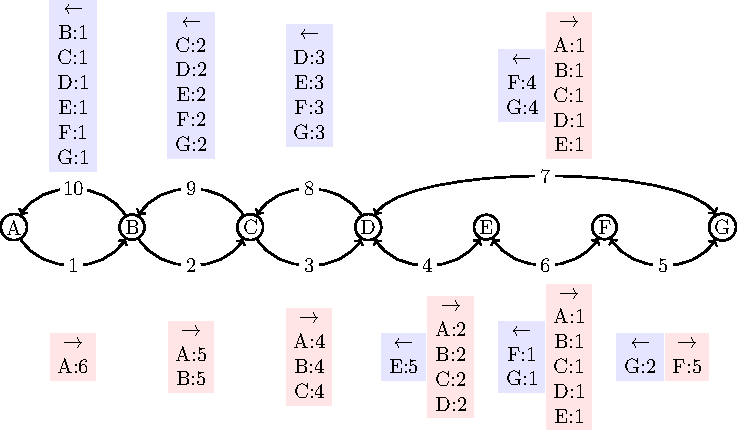
\includegraphics[width=0.6\textwidth]{./linear/linear_cookie_sharing}}

\begin{multicols}{2}

在疫情期間，
很多人都在家裡做餅乾。
但是自己做餅乾很快就變得有點無聊，
所以你想和你的朋友玩「交換餅乾」：
你們每個人都想吃到其他人做的餅乾。
% 假設你有 $n-1$ 個好朋友都在做餅乾，
% 你希望你們 $n$ 個人每個人都可以分到其他人做的餅乾一片。
但是因為疫情的緣故，
實體碰面交換餅乾的次數應該要越少越好，
那麼玩「交換餅乾」需要碰幾次面呢？

其實這個問題不是什麼疫情下的新產物。
在 1970 年代初期就出現了「八卦問題」：
如果有 $n$ 個人、每個人都有一則八卦，
那麼這 $n$ 群人之間至少要通幾次電話才能讓每個人都知道所有八卦？
	\footnote{但是因為這是 1970 年代，大家不是很在意性別刻板印象，
	所以原始的敘述其實是「有 $n$ 個女人、每個女人都有一則八卦⋯」。
	由於我不想要被 cancel，所以就把問題稍微改寫了。
	想看原始問題的話可以看看 \textcite{BAKER1972191} 裡面的描述。}
這個問題跟我們想要解決的「交換餅乾」基本的概念是一樣的，
解決了需要幾次交換之後，
每次要交換餅乾的數量就好辦了。

為了討論方便，
我們用 $f(n)$ 表示 $n$ 個人所需最少的通話數。
顯然地， $f(2)=1$ 因為 2 個人只需要交換 1 次；
而 3 個人的話不可能只交換 1 次或 2 次，所以就一定至少要 3 次，$f(3)=3$；
類似地也可以得到 $f(4)=4$；
若稍微想一下可能可以得到 $f(5)=6$，
但是當 $n$ 更大的時候要求得 $f(n)$ 就比較困難了。

多試幾次之後你會發現人數多的時候都需要差不多 $2n$ 次，
而這個觀察在直觀上也很好理解：
一則八卦傳到最後一個人後，
要再傳回來一次大家才會都知道所有八卦，
所以要經過每個人 2 次。
神奇的是，這個觀察其實已經非常地好了：
數學家證明當 $n\geq5$ 的時候 $f(n)=2n-4$；
也就是說需要比 $2n$ 次稍微少一點點，
而最後的 $-4$ 是可以透過一些末端巧妙的交換達成。
雖然 $f(n)=2n-4$ 的證明有些繁瑣，
	\footnote{可以看 \textcite{BAKER1972191} 跟 \textcite{TIJDEMAN1971} 的內容了解細節。
	在\href{https://www.math.uni-bielefeld.de/~sillke/PUZZLES/gossips.pdf}{這個網頁上}有把這兩種證明方式寫在一起。}
但是我們可以直觀地求出 $f(n)\leq2n-4$ 這個上界。

考慮 $n\geq 5$ 的情形：
假設我們知道 $f(n)$ 是多少，
如果今天多一個人 A，也就是總共變成 $n+1$ 個人的話，
最多會需要打幾次電話呢？
我們可以先讓 A 打給原本 $n$ 個人裡面其中一個，
然後那個人在 $f(n)$ 次之後就可以知道所有 $n$ 個人的八卦，
然後最後把所有聽來的八卦再轉告給 A。
如此一來只多用了兩通電話，大家也都知道所有八卦，
所以我們就有
\begin{align*}
	f(n+1) \leq f(n) + 2,
	\quad 
	n \geq 5
\end{align*}
這樣的遞迴式。
把這個遞迴式寫成一般試，再加上 $f(n)=4$ 的條件就可以得到 $f(n)\leq 2n-4$ 了。

如此一來你就知道反正大概就是需要 $2n$ 次，
剩下的工作就是考慮每個人要給下一個人幾片餅乾了。
最簡單的相法應該就是把所有餅乾都給一個人，
然後大家再去跟那個人領，
這樣就可以 $2n-3$ 次完成。
但是這樣感覺都跟同一個人接觸很多次有點危險，
所以我在圖中呈現一種無論 $n$ 為何，一個人最多只會接觸 3 個人的交換方式。
（驗證看看怎麼拓展成任意 $n$ 人的版本！無論有幾個人，只要最後 4 個人做一些比較複雜的交換，
就可以確保一個人最多只接觸 3 個人並且達到最少次的交換次數。）
而顯然地給幾片餅乾的方式並不唯一，
所以我就在圖中呈現了一個我覺得最直觀的方式。
	\footnote{圖中 A、...、G 共 7 人，
	之間連接的箭頭表示交換，箭頭上的數字表示交換的順序，
	而在塗色方匡中表示要傳幾片餅乾。
	例如在第 4 次交換中 E 會收到 D 給他 A、B、C、D 的餅乾各 2 片，
	而 D 會收到 E 給他 5 片 E 自己的餅乾。}

但是這個圖無論怎麼畫感覺就是傳染鏈的樣子啊，
所以還是不要在疫情期間玩交換餅乾好了⋯⋯
\hfill$\blacksquare$
\printbibliography[title={\normalsize{參考資料}}]
\end{multicols}
\end{document}
